\ProvidesPackage{commands}
\documentclass[11pt]{article}
\usepackage{epstopdf}
\usepackage{amsmath}
\usepackage{epsf}
\usepackage{amsfonts}
\usepackage{amssymb}
\usepackage{color}
\usepackage{mathtools}
\usepackage{placeins}
\usepackage{booktabs}
\usepackage{enumitem}
\usepackage{caption}
\usepackage[margin=0.85in, paperwidth=8.5in, paperheight=11in]{geometry}
\usepackage{amsfonts}
\usepackage{amsmath}
\usepackage{amsbsy}
\usepackage{authblk}
\usepackage{listings}
\usepackage{array}
\usepackage{titlesec}
\usepackage{amssymb}
\usepackage{bm}
\usepackage{mathtools}
\usepackage{titlesec}
\usepackage{empheq}
\usepackage[latin1]{inputenc}\newcommand{\bs}[1]{\boldsymbol{#1}}
\usepackage{mathtools}
\usepackage{graphicx}
\usepackage{caption}
\usepackage{subcaption}

\newcommand{\del}[2]{\frac{\partial {#1}}{\partial {#2}}}
\newcommand{\D}[2]{\frac{D^{\overline{\alpha}}}{\overline{\alpha !}}{#1}(#2,#2)\ {\bf x}^{\overline{\alpha}}}
\newcommand{\dv}[3]{\frac{{\rm d}^{#1}{#2}}{d{#3}^{#1}}}
\newcommand{\ddel}[5]{\frac{\partial^{ {#1} + {#2}} {#3}}{\partial {#4}^{#1} \partial{#5}^{#2}}}
\newcommand{\dev}{{\rm {\bf dev}}}
\newcommand{\proj}[1]{\frac{1}{R^2}{\bf X}\otimes{\bf X}}
\newcommand{\Ie}[1]{I^{\rm e}_{#1}}
\newcommand{\Ce}[1]{\bf C^{\rm e^{#1}}}
\newcommand{\Fe}[2]{F^{\rm e^{#2}}_{#1}}
\newcommand{\Fv}[2]{F^{\rm v^{#2}}_{#1}}
\newcommand{\C}[2]{C^{\rm {#2}}_{#1}}
\newcommand{\f}[2]{f^{\rm {#2}}_{#1}}
\newcommand{\B}[2]{B^{\rm {#2}}_{#1}}
\newcommand{\E}[2]{E^{\rm {#2}}_{#1}}
\newcommand{\fv}[2]{f^{\rm v^{#2}}_{#1}}
\newcommand{\dfv}[2]{\dot{f}^{\rm v^{#2}}_{#1}}
\newcommand{\tGam}[2]{\tilde{\Gamma}^{\rm v^{#2}}_{#1}}
\newcommand{\Gam}[2]{\Gamma^{\rm v^{#2}}_{#1}}
\newcommand{\A}[1]{\mathcal{A}_{#1}}
\newcommand{\F}[2]{F^{\rm #2}_{#1}}
\newcommand{\hpeq}{\hat{\psi}^{\rm Eq}}
\newcommand{\hpneq}{\hat{\psi}^{\rm NEq}}
\newcommand{\etak}{\eta_K({I_1,I_2,J},{\bf C^{\rm e}, B^{\rm v}})}
\newcommand{\nuk}{\nu_K({I_1,I_2,J},{\bf C^{\rm e}, B^{\rm v}})}
\newcommand{\thetak}{\theta_K({I_1,I_2,J},{\bf C^{\rm e}, B^{\rm v}})}
\newcommand{\etaj}{\eta_J({I_1,I_2,J},{\bf C^{\rm e}, B^{\rm v}})}
\newcommand{\dFv}[2]{\dot{F}^{\rm v^{#2}}_{#1}}
\newcommand{\hatpsi}{\widehat{\psi}(I_1, I_2,I^{\rm e}_1,I^{\rm e}_2,J)}
\newcommand{\hpsi}{\widehat{\psi}(I_1,I^{\rm e}_1,J)}
\newcommand{\Fh}[1]{\widehat{\mathcal{F}}\left({\bf F, \Fv{}{}}, {#1}\right)}
\newcommand{\Fhstar}[1]{\widehat{\mathcal{F}}^*\left({\bf F, \Fv{}{}}, {#1}\right)}
\newcommand{\sbar}{\overline{\bm{\sigma}}}
\newcommand{\hpsicomp}[1]{\sum_{r=1}^{2}\left\{\frac{3^{1-\alpha_r}}{2\alpha_r}\mu_r(I^{\alpha_r}_1-3^{\alpha_r})
+\frac{3^{1-a_r}}{2a_r}m_r({\Ie{1}}^{^{a_r}}-3^{a_r})\right\}
+\mu{#1}+\kappa{#1}^2}
\newcommand{\Ni}[1]{N^{(e)}_i(#1)}
\newcommand{\hNi}[1]{\hat{{N}}^{(e)}_i(#1)}
\newcommand{\Ld}{L^{\dagger}}
\newcommand{\intinfinf}{\int_{-\infty}^{\infty} \int_{-\infty}^{\infty}}
\newcommand{\LLnorm}[1]{\left\lVert{#1}\right\rVert_2}
\newcommand{\Linorm}[1]{{\left\lVert{#1}\right\rVert_\infty}}
\newcommand{\tr}{\rm tr}
\newcommand{\deldel}[2]{\frac{\partial^2 {#1}}{\partial {#2}^2}}
\newcommand{\kd}[1]{\delta_{#1}}
\newcommand{\Fie}[1]{{\bf F}^{#1}}
\newcommand{\Comp}{\emph{CompStrainStress\_Cee570.m}}
\newcommand{\Comps}{\emph{CompStrainStress\_Elem\_Cee570.m}}
\newcommand{\Feap}{\emph{FEA\_Program.m}}
\newcommand{\Elast}{\emph{Elast2d\_Elem.m}}
\newcommand{\Assem}{\em{AssemStifForc.m}}
\newcommand{\Fb}{\em{F\_bar\_int}}
\newcommand{\Form}{\em{FormFE.m}}
\newcommand{\Sol}{\em{SolveFE.m}}
\newcommand{\inpt}{\em{triangtwo.m}}
\newcommand{\dis}[2]{d^{{#2}}_{#1}}
\newcommand{\vel}[2]{v^{{#2}}_{#1}}


\newcommand\myeq{\stackrel{\mathclap{\normalfont\mbox{def}}}{=}}


% Matrix Spacing: 
\makeatletter
\renewcommand*\env@matrix[1][\arraystretch]{%
  \edef\arraystretch{#1}%
  \hskip -\arraycolsep
  \let\@ifnextchar\new@ifnextchar
  \array{*\c@MaxMatrixCols c}}
\makeatother

\titlespacing\section{10pt}{10pt plus 4pt minus 2pt}{10pt plus 2pt minus 2pt}
\titlespacing\subsection{0pt}{8pt plus 4pt minus 2pt}{8pt plus 2pt minus 2pt}
\titlespacing\subsubsection{0pt}{12pt plus 4pt minus 2pt}{6pt plus 2pt minus 2pt}
\titlespacing*{\title}{-2ex}{*-2ex}{-2ex}
\usepackage{color} %red, green, blue, yellow, cyan, magenta, black, white
\definecolor{mygreen}{RGB}{28,172,0} % color values Red, Green, Blue
\definecolor{mylilas}{RGB}{170,55,241}
\setlength\parindent{0pt}
\graphicspath{{Figures/}}

\usepackage{graphicx}
\title{\bf CEE 576: Nonlinear Finite Elements \\ Final Examination}
\author{Bhavesh Shrimali \\ NetID: bshrima2}
\date{\today}
\begin{document}
\maketitle \hrule\hrule\hrule
\section*{Problem 1: Initial-Boundary Value Problem}
\subsection*{Strong and Weak Forms: }
The initial boundary value problem can be formulated as follows: 
\begin{align*}
{\rm div} 
{\bm \sigma} ({\bf x},t)
+ 
{\bf f}({\bf x},t)
=
\rho\ {\bf \ddot{u}} ({\bf x},t) \ \ \ \ \ \ \ \forall \ \ \ \left\{{\bf x},t\right\}\  & \in\  \Omega\  {\rm X}\  (0,T) \\
{\bf u} ({\bf x},t) = {\bf g}({\bf x},t) \ \ \ \ \ \ \ \forall \ \ \ \left\{ {\bf x},t \right\}\ & \in\ \Gamma_g\  {\rm X}\  (0,T)\\
{\bf t} ({\bf x},t)
=
{\bm\sigma}\cdot{\bf n}
= 
{\bf h}({\bf x},t)
 \ \ \ \ \ \ \ \forall \ \ \ \left\{ {\bf x},t \right\}\ & \in\ \Gamma_h\  {\rm X}\  (0,T)
\end{align*}
subject to initial conditions: 
\begin{align*}
{\bf u}
({\bf x},0)
 =
 {\bf u}_{_0} ({\bf x}_{_0})  \ \ \ \ \ \ \ \forall \ \ \ \left\{ {\bf x} \right\}\ & \in\ \Omega_0 \\
 \dot{\bf u}
({\bf x},0)
 =
 \dot{\bf u}_{_0} ({\bf x}_{_0})  \ \ \ \ \ \ \ \forall \ \ \ \left\{ {\bf x} \right\}\ & \in\ \Omega_0
\end{align*}
The above is the spatial description of the governing equations. The spatial discretization of the problem is achieved by working out the Weak-form and introducing piece-wise continuous functions. This is done as follows: 
\begin{align*}
\int_{\Omega}
{\bf w}
\left(
- \rho\ddot{\bf u}
+ {\rm div} 
{\bm \sigma} ({\bf x},t)
+ 
{\bf f}({\bf x},t)
\right)\ d\Omega
\end{align*} 
We rewrite the above equation in the indicial notation, and ignore the arguments for brevity: 
\begin{align*}
\int_{\Omega}
w_i
\left(
- \rho \deldel{u_i}{t}
+ 
\del{\sigma_{ij}}{x_j}
+ f_i
\right)\ 
d\Omega
=
0
\end{align*} 
Using divergence theorem on the second term and denoting the velocity in the current configuration by $v_i = \dot{u}_i$,  we get
\begin{align*}
& \mathbb{A}_e\ 
 \int_{\Omega_e}
w_i
\left(
-\rho\del{v_i}{t} + 
\del{}{x_j}
\left(
w\sigma_{ij}
\right)
-
\del{w_i}{x_j}\sigma_{ij}
+
w_i \cdot f_i
\right)
\ d\Omega\ 
=0 \\
& \mathbb{A}_e\  
\left( 
\int_{{\Omega_e}}
w_i\  \rho\  \del{v_i}{t}
+
\del{w_i}{x_j}\sigma_{ij} \ d\Omega
\right)
=
\mathbb{A}_e\ 
\left( 
\int_{{\Omega_e}}
w_i\cdot f_i \ d\Omega
+
\int_{{\Gamma_h}}
w_i\ \sigma_{ij}\ d\Gamma
\right)
\end{align*}
where $\mathbb{A}_e$ denotes the assembly operation over all the elements. The respective integrals can further be evaluated using a standard Gaussian-Quadrature rule. 
\begin{align*}
\mathbb{A}_e\  
\left( 
\int_{{\boxed{}}}
w_i\  \rho\  \del{v_i}{t}
+
\del{w_i}{x_j}\sigma_{ij}
\right)
=
\mathbb{A}_e\ 
\left( 
\int_{{\boxed{}}}
w_i\cdot f_i \ d\Omega
+
\int_{{\Gamma_h}}
w_i\ \sigma_{ij}\ d\Gamma
\right)
\end{align*}
where $\int_{\boxed{}}$ denotes the integral over the canonical domain. And further ($q_i$) denote the weights
\begin{align*}
\boxed{\mathbb{A}_e\  
\sum_{\xi_i} \cdot J({\bf x},{\bf\xi})\cdot q_i\cdot
\left( 
w_i\  \rho\  \del{v_i}{t}
+
\del{w_i}{x_j}\sigma_{ij}
\right)
=
\mathbb{A}_e\ 
\left( 
\sum_{\xi_i}\cdot J({\bf x},{\bf\xi})\cdot q_i\cdot
w_i\cdot f_i 
+
\int_{{\Gamma_h}}
w_i\ \sigma_{ij}\ d\Gamma
\right)}
\end{align*}
The corresponding space of functions is : 
\begin{align*}
\boxed{
\begin{aligned}
& u_i \in \mathcal{S} : \ \ \forall w_i \in \mathcal{V} \\
& \mathcal{S} = 
\begin{Bmatrix}
u & |\ u_i \in \mathcal{H}^1 (\Omega) & u_i = g_i \ \ \text{on}\ \ \Gamma_{g_i}
\end{Bmatrix} \ \ \ \text{and} \ \ \ 
\mathcal{V} = 
\begin{Bmatrix}
v & |\ v_i \in \mathcal{H}^1 (\Omega) & v_i = 0 \ \ \text{on}\ \ \Gamma_{g_i}
\end{Bmatrix}
\end{aligned}
}
\end{align*}
\subsection*{\underline{Matrix Form: }}
The corresponding Matrix form would be
\begin{align*}
{\bf M}\ddot{\bf d}
+
{\bf N}({\bf d})
=
{\bf f}_{\rm ext}
\end{align*}
where the corresponding mass matrix can be developed as follows: 
\begin{align*}
{\bf M}
=
\mathbb{A}_e\ \int_{\Omega_e}
{\bf N}^T \rho \ {\bf N}\ d\Omega
\end{align*}
This can be developed as follows : (Note that ${\bf F}^i$ denotes the inertial force) 
\begin{align*}
{\bf F}^{i}
& = 
\mathbb{A}_e\ 
\int_{\Omega}
{\bf w}^{\rm e^{T}}\ \rho
\ddot{\bf u}\ d\Omega \\
{\bf w}^{\rm e^{T}}
& =
\left(
{\bf N}^e_a\ \delta {\bf d}^e_a
\right)^T \ \ ; \ \ \ \ \ddot{\bf u} = 
\left(
{\bf N}^e_b\ \ddot{\bf d}^e_b
\right)
\end{align*}
Substituting we get : 
\begin{align*}
{\bf F}^i
=
\mathbb{A}_e\ {\bf F}^i_e
=
\mathbb{A}_e
\ 
{\delta {\bf d}^e_a}^T \left(
\int_{\Omega_e}
{\bf N}^e_a\ \rho\ {\bf N}^e_b\ d\Omega \right)\ddot{\bf d}^e_b = \mathbb{A}_e
\ 
{\delta {\bf d}^e_a}^T {\bf M}^e_{ab}\ \ddot{\bf d}^e_b
\end{align*}
Hence the Mass Matrix is given by: 
\begin{align*}
\boxed{{\bf M}^e_{ab}
=
\int_{\Omega_e}
{\bf N}^e_a\ \rho\ {\bf N}^e_b\ d\Omega 
}
\end{align*}\hrule
\newpage\subsection*{(c) Consistent Tangent : }
The consistent tangent can be derived using the process of consistent linearization as follows: 
\begin{align*}
\mathcal{F}(\varphi)
=
\int_{\Omega}
w_{i,j}
\sigma_{ij} ({\bf \varphi})\ d\Omega
=
\int_{\Omega_0}
W_{i,I}P_{iI}\ d\Omega_0
=
\int_{\Omega_0}
W_{i,I}F_{iJ}S_{IJ}\ d\Omega_0
=
\del{W}{X_I}\del{\varphi_i}{X_J}S_{_{JI}} d\Omega_0
\end{align*}
Taking the Taylor-Expansion of the integral we get: 
\begin{align*}
\del{}{\varepsilon}\mathcal{F}
\left(
\bm\varphi + \varepsilon\Delta {\bf u}
\right)|_{\varepsilon =  0} \ \ \  & \myeq\ \ \  \mathbb{D}\mathcal{\bm\varphi}\cdot \Delta {\bf u} \ \ \ \text{for }\ \ \ \varepsilon \in \mathbb{R}
\end{align*}
Now
\begin{align*}
\mathcal{F}
(\bm\varphi + \varepsilon\Delta {\bf u})
& =
\int_{\Omega_0}
W_{i,I}
\del{}{X_J}
(\bm\varphi + \varepsilon\Delta {\bf u})\ S_{IJ}\ 
({\bf E}(\bm\varphi + \varepsilon\Delta {\bf u}))\ d\Omega_0 \\
\mathbb{D}\ 
\mathcal{F}({\bm\varphi})
\cdot{\bf u}
& =
\int_{\Omega_0}
W_{i,I}
\left(
\del{\Delta u_i}{X_J}\right)
\ S_{IJ}\ ({\bf E}({\bm\varphi}))\ d\Omega_0\  + 
\int_{\Omega_0}
W_{i,I}
\del{\varphi_i}{X_J}\del{S_{IJ}}{E_{KL}} \left( 
\del{E_{KL}}{\varepsilon}
\left(
\bm\varphi 
+
\varepsilon \Delta{\bf u}
\right)
\right)\bigg|_{\varepsilon = 0}d\Omega_0 \\
& = 
W_{i,I}
\left(
\del{\Delta u_i}{X_J}\right)
\ S_{IJ}\ ({\bf E}({\bm\varphi}))\ d\Omega_0\ +
\int_{\Omega_0}
W_{i,I}\left(
\del{\varphi_i}{X_J}\right) {\mathbb{C}}_{IJKL}\left( 
\del{E_{KL}}{\varepsilon}
\left(
\bm\varphi 
+
\varepsilon \Delta{\bf u}
\right)
\right)\bigg|_{\varepsilon = 0}d\Omega_0 
\end{align*}
We also know
\begin{align*}
{\bf E}
& =
\frac{1}{2}
\left(
{\bf \F{}{T}\F{}{} - I}
\right)\\
\implies 
{\bf E}
\left(
\varphi + \varepsilon\Delta{\bf u}
\right)
& =
\frac{1}{2}
\left(
\del{}{\bf X}
\left(
\varphi + \varepsilon\Delta{\bf u}
\right)
\del{}{\bf X}
{
\left(
\varphi + \varepsilon\Delta{\bf u}
\right)
}^T - {\bf I}
\right)
\end{align*}
Evaluating the above expression: 
\begin{align*}
2\del{E_{KL}}{\varepsilon}|_{\bm\varepsilon = 0}
& =
\Delta u_{j,k} \phi_{j,L} + \phi_{j,K}\Delta u_{j,L} \\
& = 
\Delta u_{j,k}F_{jL}
+
F_{jk}\Delta u_{j,L} \\
& \del{}{\varepsilon}
(E_{KL})|_{\varepsilon = 0}
=
\frac{1}{2}
\left(
\Delta u_{j,k}F_{jL} + F_{jK}\Delta u_{j,L}
\right)
\end{align*}
Employing the use of minor symmetry to get: 
\begin{align*}
\mathbb{D}\mathcal{F}(\phi)\cdot\Delta {\bf u}
=
\int_{V}
\left(
W_{i,I}\Delta u_{i,J}S_{JI} ({\bf E}(\phi)) + W_{i,I}F_{iJ}F_{jL}\mathbb{C}_{IJKL}\Delta u_{j,k}
\right)\ dV
\end{align*}
Ignoring the arguments for all the terms explicitly in the above expression. To this end, we recall, 
\begin{align*}
& d\ {\rm v} = J\ dV \\
& W_{i,I} = w_{i,k}\ F_{kI} \\
& \Delta U_{i,k}
=
\Delta
u_{i,k}F_{kK}
\end{align*}
The first term in the previous integral can therefore be rewritten as : 
\begin{align*}
& \int_{\rm v}
w_{i,k}
\left(
J^{-1}
F_{kI}
F_{jI}
S_{JI}
\right)
\Delta u_{i,j}\ d{\rm v} = \int_{\rm v} w_{i,k} \sigma_{kj}\Delta u_{i,j}\ d{\rm v}
\end{align*}
and correspondingly the second term: 
\begin{align*}
\int_{\rm V}
& W_{i,I}F_{iJ}F_{jL}\mathbb{C}_{IJKL}\Delta u_{j,k}\ d{\rm V} = \int_{\rm v}
w_{i,j}\ c_{ijkl}\ \Delta u_{k,l}\ d{\rm v}
\end{align*}\hrule
\section*{Problem 2: Consistent Mass Matrix}
\subsection*{(a) : Weak Form --- Mass Matrix}
Given reference density distribution : 
\begin{align*}
\rho_0
=
1.0
+
\frac{Y}{50}
\end{align*}
Using the formulation developed in the Problem 1, we have \begin{align*}
{\bf M}
=
\mathbb{A}_e\ \int_{\Omega_e}
{\bf N}^T \rho \ {\bf N}\ d\Omega
\end{align*}
This can be developed as follows : (Note that ${\bf F}^i$ denotes the inertial force) 
\begin{align*}
{\bf F}^{i}
& = 
\mathbb{A}_e\ 
\int_{\Omega}
{\bf w}^{\rm e^{T}}\ \rho
\ddot{\bf u}\ d\Omega \\
{\bf w}^{\rm e^{T}}
& =
\left(
{\bf N}^e_a\ \delta {\bf d}^e_a
\right)^T \ \ ; \ \ \ \ \ddot{\bf u} = 
\left(
{\bf N}^e_b\ \ddot{\bf d}^e_b
\right)
\end{align*}
Substituting we get : 
\begin{align*}
{\bf F}^i
=
\mathbb{A}_e\ {\bf F}^i_e
=
\mathbb{A}_e
\ 
{\delta {\bf d}^e_a}^T \left(
\int_{\Omega_e}
{\bf N}^e_a\ \rho\ {\bf N}^e_b\ d\Omega \right)\ddot{\bf d}^e_b = \mathbb{A}_e
\ 
{\delta {\bf d}^e_a}^T {\bf M}^e_{ab}\ \ddot{\bf d}^e_b
\end{align*}
Hence the Mass Matrix is given by: 
\begin{align*}
\boxed{{\bf M}^e_{ab}
=
\int_{\Omega_e}
{\bf N}^e_a\ \rho\ {\bf N}^e_b\ d\Omega 
}
\end{align*}\hrule
\subsection*{(b) Consistent Mass Matrix :}
Now we know here that
\begin{align*}
{\bf N}
=
\left< 
N_1 \ N_2 \ N_3 \ N_4 
\right> = 
\frac{1}{4}
\left< 
(1-\xi)(1-\eta)\ (1+\xi)(1-\eta)\ (1+\xi)(1+\eta)\ (1-\xi)(1+\eta)\ 
\right>
\end{align*}
Here the node numbering is done such that the node corresponding to the lowest global node number is assigned the local node 1, the second lowest 2 and so on. Also we assume the same degree of interpolation for each direction, and therefore have: 
\begin{align*}
{\bf M}^e
& =
\int_{\Omega_e}
{\bf N}^T_a\ \rho {\bf N}_b\ d\Omega = 
\int_{-1}^1 \int_{-1}^1
\begin{bmatrix}
N_1 & 0 \\
0 & N_1 \\
N_2 & 0 \\
0 & N_2 \\
N_3 & 0 \\
0 & N_3 \\
N_4 & 0 \\
0 & N_4 
\end{bmatrix}\cdot \rho (\eta) \cdot
\begin{bmatrix}
N_1 & 0 & N_2 & 0 & N_3 & 0 & N_4 & 0 \\
0 & N_1 & 0 & N_2 & 0 & N_3 & 0 & N_4  
\end{bmatrix}\ J({\bf x},{\bf\eta})\ d\xi\ d\eta
\end{align*}
The above integral is computed using 2-point Gauss Quadrature in each direction, for which the weights and the Gauss-points are given as follows: 
\begin{align*}
W_i = \begin{Bmatrix}
1 & 1 \\ 1& 1
\end{Bmatrix} \ \ ; \ \ \ \ \ \ 
({\bf \xi,\eta}) = \frac{1}{\sqrt{3}}
\begin{bmatrix}
-1 & 1\\ -1 & 1 
\end{bmatrix} 
\end{align*}
\begin{align*}
\rho (\eta) =
\frac{1+\eta}{100} +1
\end{align*}
Substituting we get : 
\begin{align*}
{\bf M}^e = 
\begin{bmatrix}
 0.1117      &   0    &0.0558      &   0    &0.0281        & 0  &  0.0561   &      0 \\
         0   & 0.1117      &   0  &  0.0558 &        0  &  0.0281    &     0  &  0.0561 \\
    0.0558  &       0   & 0.1117    &     0  &  0.0561  &      0   & 0.0281     &    0 \\
         0  &  0.0558   &      0   & 0.1117   &      0  &  0.0561    &     0  &  0.0281 \\
    0.0281   &      0  &  0.0561    &     0 &   0.1128    &     0  &  0.0564  &       0 \\
         0 &   0.0281 &        0  &  0.0561   &      0  &  0.1128     &   0  &  0.0564 \\
    0.0561  &       0 &   0.0281  &       0   & 0.0564    &     0  &  0.1128  &       0 \\
         0  &  0.0561  &       0   & 0.0281 &        0  &  0.0564      &   0   & 0.1128
\end{bmatrix}
\end{align*}\hrule
\subsection*{(c) Row Sum Technique}
Using the row sum technique we get the corresponding diagonal mass matrix as follows: 
\begin{align*}
{\bf M}^e_l
\begin{bmatrix}
 0.2517 &    0  &   0  &   0  &   0  &   0  &   0  &   0\\
     0  &   0.2517   &  0   &  0   &  0   &  0   &  0   &  0\\
     0  &   0   &  0.2517   &  0   &  0   &  0   &  0   &  0\\
     0  &   0   &  0   &  0.2517   &  0   &  0   &  0   &  0\\
     0  &   0   &  0   &  0   &  0.2533   &  0   &  0   &  0\\
     0  &   0   &  0   &  0   &  0   &  0..2533   &  0   &  0\\
     0  &   0   &  0   &  0   &  0   &  0   &  0.2533   &  0\\     
     0  &   0   &  0   &  0   &  0   &  0   &  0   &  0.2533     
\end{bmatrix}
\end{align*}\hrule
\section*{Problem 3: Discretization and Numerical Implementation}
The equation of motion as obtained in the problem (1) is the starting equation upon which the generalized alpha ($\alpha$) method is applied, i.e.: 
\begin{align*}
{\bf M} \ddot{\bf d}
=
(1+\alpha)
\left(
\bf\F{n+1}{ext} - \F{n+1}{int}
\right)
- \alpha 
\left(
\bf\F{n}{ext} - \F{n}{int}
\right)
\end{align*}
Now, since all the above quantities are at the current iterate, i.e., $t_{n+1}$ we linearize the second term in the expansion as follows: 
\begin{align*}
{\bf \F{n+1}{int}}
=
{\bf N}({\bf d}_{n})
+
\del{\bf N}{\bf d}({\bf d}_n) \cdot\Delta {\bf d} = 
{\bf N}({\bf d}_{n})
+
{\bf K}({\bf d}_n) \cdot\Delta {\bf d} = 
\end{align*}
The initial value of the displacement and velocity are prescribed and hence we march forward in time, using the recurrence relation specified by the generalized alpha method described above and proceed with defining the predictors 
\begin{align*}
\tilde{\bf d}_{n+1}
=
{\bf d}_{n}
+
\Delta t {\bf v}_n
+ \frac{\Delta t^2}{2} (1-2\beta){\bf a}_n \ \ ; \ \ \ \ \ \ 
\tilde{\bf v}_{n+1}
=
{\bf v}_n
+
(1-\gamma)\Delta t {\bf a}_n
\end{align*}
where the time integration parameters are as defined below: 
\begin{align*}
\beta = \frac{(1-\alpha)^2}{4} \ \ ; \ \ \ \ \ \ \gamma = \frac{1-2\alpha}{2}
\end{align*}
We substitute these back into the equation of motion to arrive at: 
\begin{align*}
{\bf M}^*\ \cdot {\bf \Delta d} = {\bf R}_{n+1-\alpha}
\end{align*}
where again
\begin{align*}
{\bf M}^*
=
\frac{\bf M}{\beta\Delta t^2} + (1+\alpha){\bf K} \ \ ; \ \ \ \ \ \ \ 
{\bf R}_{n+1-\alpha}
=
(1+\alpha)
\left(
\bf\F{n+1}{ext} - {\bf N}({\bf d}_{n+1})
\right)
- \alpha 
\left(
\bf\F{n}{ext} - {\bf N}({\bf d}_n)
\right) - {\bf M} {\bf a}_n
\end{align*}
After making one-pass through the algorithm to solve the above linearized system for the incremental displacements we apply the correctors as follows: 
\begin{align*}
\boxed{{\bf d}^{i+1}_{n+1}
=
{\bf d}^i_{n+1} + \Delta {\bf d} \ \ ; \ \ \ \ \ 
{\bf a}^{i+1}_{n+1}
=
\frac{{\bf d}^{i+1}_{n+1} - {\bf d}_n - \Delta t {\bf v}_n}{\beta\Delta t^2}
-
\left(
\frac{1-2\beta}{2\beta}
\right) {\bf a}_n \ \ ; \ \ \ \ {\bf v}^{i+1}_{n+1}
=
{\bf v}^i_n
+ 
\Delta t
(\gamma {\bf a}^{i+1}_{n+1} + (1-\gamma){\bf a}_n)}
\end{align*}
The correctors are applied at each iteration, until convergence is met within an admissible tolerance (specified in the input file). The corresponding flow-chart is attached at the end, after the required plots. 
\section*{Problem 4: Plots and Comments}
The corresponding plots are attached below: 
\subsection*{(a): Axial Tension }
For the case of axial tension at the nodes (3) and (4) a quasi-static computation is done beforehand to specify a displacement in the y-direction of magnitude equal to 0.2 units. The obtained plots for the case of the parameter ($\alpha = 0$) and ($\alpha = -1/3$) are as follows: 
\begin{figure}[h!]
\centering
\begin{subfigure}{.5\textwidth}
  \centering
  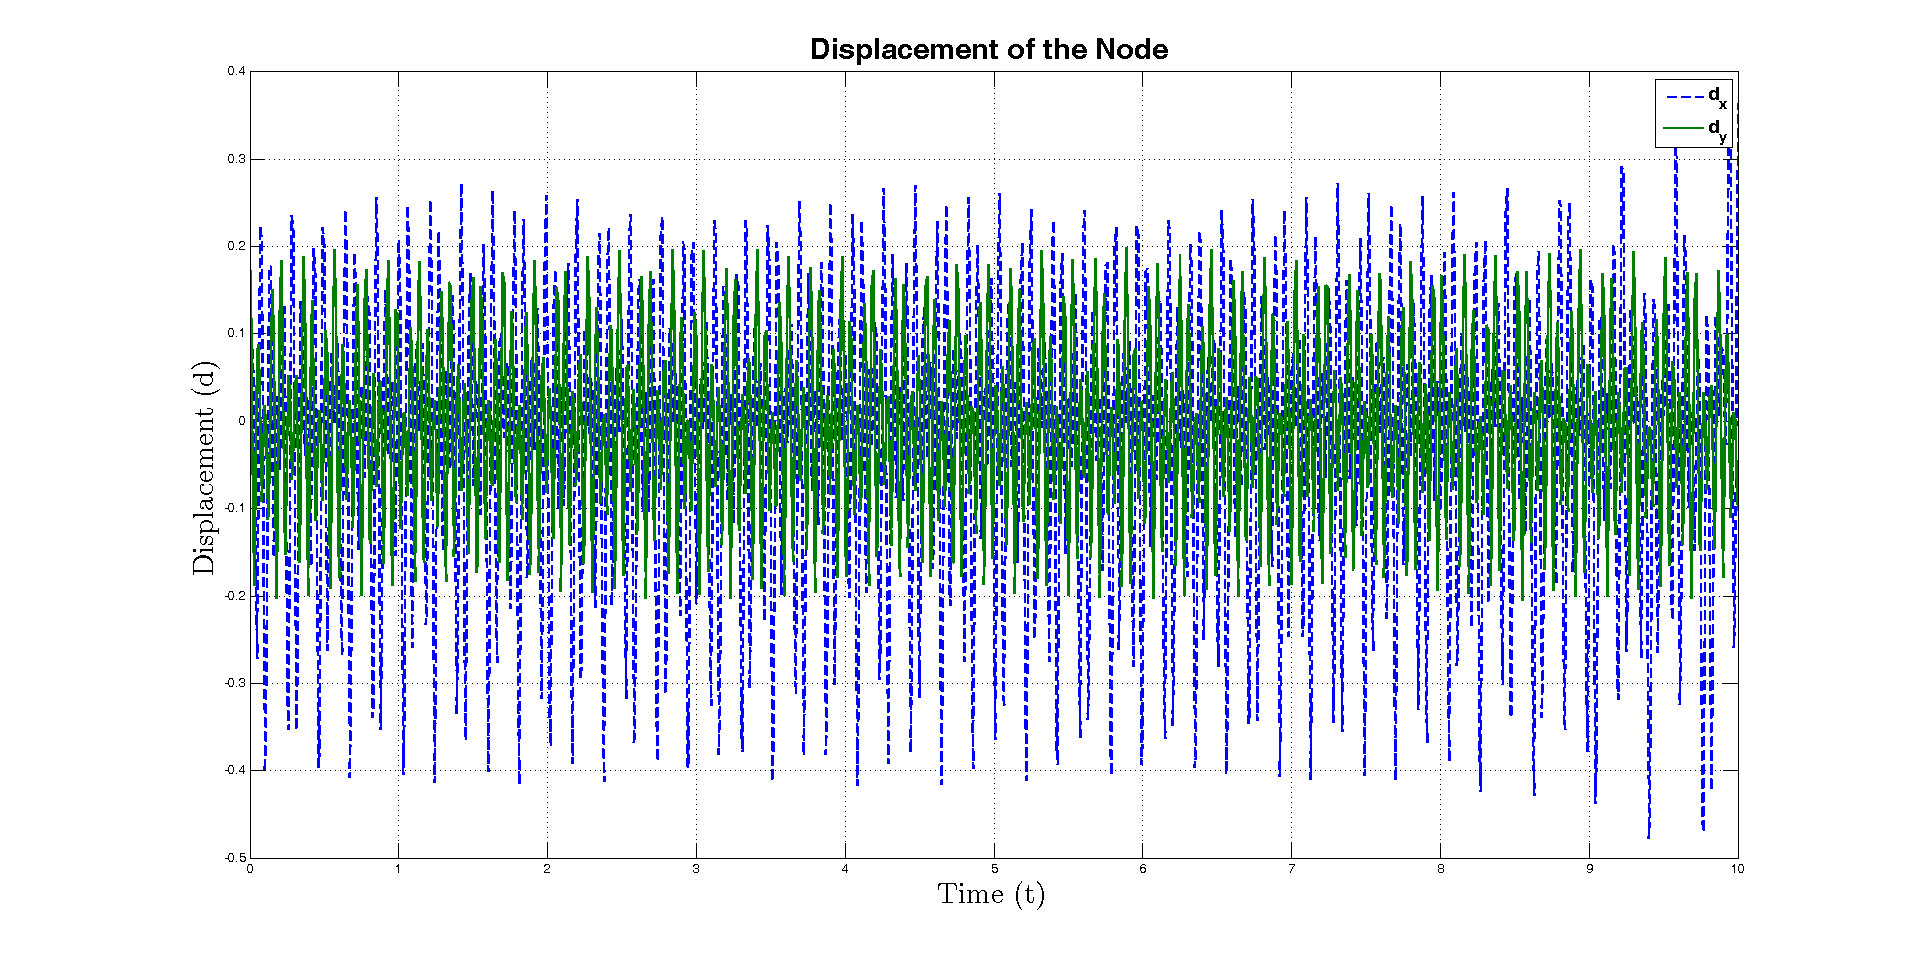
\includegraphics[width=4in,height = 4in]{dis4ai}
  \caption{N = 100}
  \label{fig:sub1}
\end{subfigure}%
\begin{subfigure}{.5\textwidth}
  \centering
  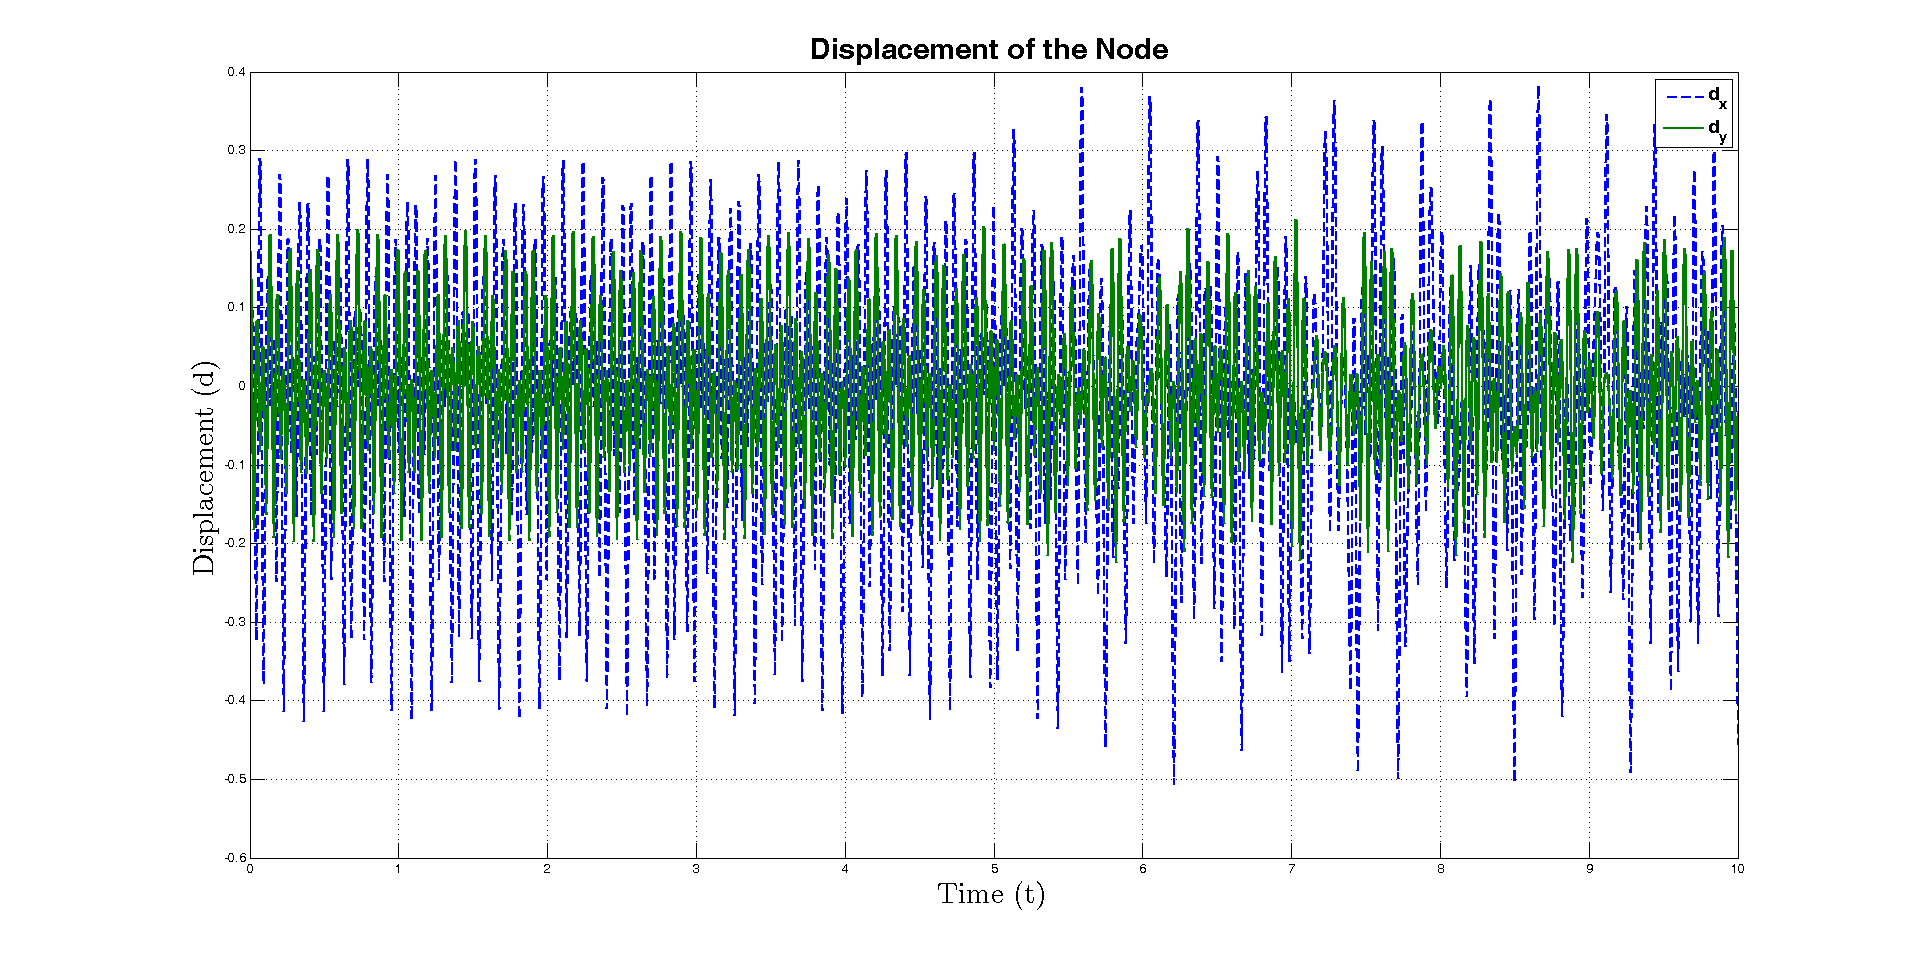
\includegraphics[width=4in,height = 4in]{dis4aii}
  \caption{N = 200}
  \label{fig:sub2}
\end{subfigure}
\caption{ Displacement-Time Plots for Axial Tension at Node (3) }
\label{Axial-Tension}
\end{figure}\hrule
\end{document}